\documentclass[aspectratio=169]{beamer}

\usepackage[utf8]{inputenc}
\usepackage[english]{babel}
\usepackage{booktabs}
\usepackage{array}
\usepackage{listings}
\usepackage{tikz}
\usetikzlibrary{arrows.meta,positioning,shapes.geometric,calc}

\graphicspath{{logo/}{../logo/}}

\definecolor{ForestGreen}{RGB}{22,100,70}
\definecolor{SoftGreen}{RGB}{229,244,235}
\definecolor{SoftBlue}{RGB}{226,239,255}
\definecolor{SoftOrange}{RGB}{255,241,220}
\definecolor{SoftPurple}{RGB}{239,231,255}

\newcolumntype{L}[1]{>{\raggedright\arraybackslash}p{#1}}

\mode<presentation>{
  \usetheme{Ilmenau}
  \usecolortheme{spruce}
  \usefonttheme{professionalfonts}
  \setbeamertemplate{navigation symbols}{}
  \setbeamertemplate{headline}{}
  \setbeamertemplate{caption}[numbered]
  \setbeamercolor{institute in head/foot}{fg=ForestGreen}
}

\lstdefinestyle{py}{
  language=Python,
  basicstyle=\ttfamily\scriptsize,
  keywordstyle=\color{blue!75!black}\bfseries,
  commentstyle=\color{gray!80!black},
  showstringspaces=false,
  keepspaces=true,
  columns=fullflexible,
  breaklines=true,
  frame=single,
  rulecolor=\color{ForestGreen!60},
  backgroundcolor=\color{SoftBlue!35},
  tabsize=4
}

\tikzset{
  process/.style={draw=ForestGreen,rounded corners,fill=SoftGreen,thick,
    minimum height=0.9cm,text width=2.7cm,align=center},
  smallbox/.style={draw=ForestGreen,rounded corners,fill=SoftGreen,thick,
    minimum height=0.82cm,text width=2.4cm,align=center},
  arrow/.style={-Latex,very thick,ForestGreen}
}

\title[TOKT11105 -- Lecture 5]{Data Structures and Algorithms in Python\\
Lecture 5: Data Structures}
\subtitle{Part 1: Data Structures as ADTs\\Operations, Abstractions, and Python Implementations}
\author{Faculty of Data Science and Artificial Intelligence}
\institute{National Economics University}
\date{}

\begin{document}

\begin{frame}[plain]
  \setbeamercolor{block body example}{bg=ForestGreen,fg=white}
  \begin{center}
    \begin{beamercolorbox}[wd=\textwidth,sep=1pt,center,rounded=true,shadow=true]{block body example}
      \IfFileExists{logo_slide.png}{\includegraphics[width=0.27\textwidth]{logo_slide.png}}{{\vspace{0.7em}\Large\bfseries FDA -- NEU\vspace{0.7em}}}
    \end{beamercolorbox}
  \end{center}
  \vspace{-0.25em}
  \titlepage
\end{frame}

\logo{\IfFileExists{logo_fda.png}{\includegraphics[width=0.8cm]{logo_fda.png}}{}}
\setbeamercolor{footline upper}{bg=ForestGreen!22,fg=ForestGreen!85!black}
\setbeamercolor{footline lower}{bg=ForestGreen,fg=white}
\setbeamertemplate{footline}{%
  \leavevmode
  \hbox{%
    \begin{beamercolorbox}[wd=.50\paperwidth,ht=2.35ex,dp=.75ex,
      leftskip=1em]{footline upper}
      Faculty of Data Science and Artificial Intelligence
    \end{beamercolorbox}%
    \begin{beamercolorbox}[wd=.50\paperwidth,ht=2.35ex,dp=.75ex,
      rightskip=1em plus1fil]{footline upper}
      \hfill National Economics University
    \end{beamercolorbox}%
  }
  \hbox{%
    \begin{beamercolorbox}[wd=.72\paperwidth,ht=2.35ex,dp=.75ex,
      leftskip=1em]{footline lower}
      \insertshorttitle
    \end{beamercolorbox}%
    \begin{beamercolorbox}[wd=.28\paperwidth,ht=2.35ex,dp=.75ex,
      rightskip=1em plus1fil]{footline lower}
      \hfill Slide \insertframenumber/\inserttotalframenumber
    \end{beamercolorbox}%
  }
}

\begin{frame}{Part 1 roadmap}
\small
\begin{columns}[T,onlytextwidth]
\begin{column}{0.31\textwidth}
\begin{block}{1. Operations}
What do we need to do with the data?
\begin{itemize}
  \item access, search
  \item insert, delete, update
  \item traverse, min/max
\end{itemize}
\end{block}
\end{column}
\begin{column}{0.31\textwidth}
\begin{exampleblock}{2. ADTs}
Describe behavior before implementation.
\begin{itemize}
  \item sequence, map, set
  \item stack, queue, deque
  \item tree-based structures
\end{itemize}
\end{exampleblock}
\end{column}
\begin{column}{0.31\textwidth}
\begin{alertblock}{3. Python tools}
Select a concrete implementation.
\begin{itemize}
  \item \texttt{list}, \texttt{dict}, \texttt{set}
  \item \texttt{deque}, \texttt{heapq}
  \item explicit node classes
\end{itemize}
\end{alertblock}
\end{column}
\end{columns}
\end{frame}

\begin{frame}{What is a data structure?}
\small
\begin{block}{Core definition}
A data structure organizes data so that particular operations can be performed correctly and efficiently.
\end{block}
\vspace{0.3em}
\begin{center}
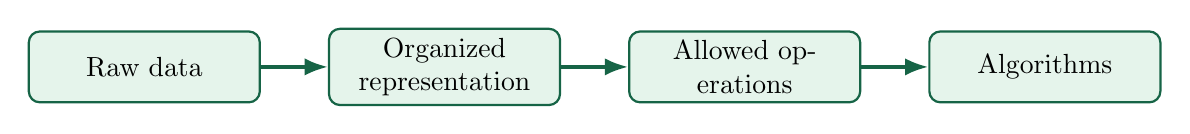
\begin{tikzpicture}[node distance=0.85cm]
  \node[process] (raw) {Raw data};
  \node[process,right=of raw] (rep) {Organized representation};
  \node[process,right=of rep] (ops) {Allowed operations};
  \node[process,right=of ops] (alg) {Algorithms};
  \draw[arrow] (raw) -- (rep);
  \draw[arrow] (rep) -- (ops);
  \draw[arrow] (ops) -- (alg);
\end{tikzpicture}
\end{center}
\vspace{0.3em}
\begin{alertblock}{Design question}
Do not ask only ``Where can I store the values?'' Ask: ``Which operations must be efficient for my workload?''
\end{alertblock}
\end{frame}

\begin{frame}{Common operations on data structures}
\scriptsize
\begin{center}
\renewcommand{\arraystretch}{1.18}
\begin{tabular}{L{0.18\textwidth}L{0.34\textwidth}L{0.34\textwidth}}
\toprule
\textbf{Operation} & \textbf{Question} & \textbf{Example} \\
\midrule
Access / retrieve & Which item is at position or key? & \texttt{A[i]}, \texttt{records[id]} \\
Search & Does a value or key exist? & find a target, membership test \\
Insert & Add a new item & append, enqueue, insert node \\
Delete & Remove an item & pop, dequeue, remove node \\
Update & Change an existing value & change grade for a student ID \\
Traverse & Visit every item & print all records, sum values \\
Min / max & Find an extreme item & smallest key, highest priority \\
\bottomrule
\end{tabular}
\end{center}
\begin{alertblock}{Main idea}
The same operation can have very different costs under different representations.
\end{alertblock}
\end{frame}

\begin{frame}{ADT: behavior before implementation}
\small
\begin{block}{Abstract Data Type (ADT)}
An ADT specifies the values, the allowed operations, and the required behavior of those operations. It does not specify how the values are stored in memory.
\end{block}
\begin{center}
\renewcommand{\arraystretch}{1.2}
\begin{tabular}{L{0.20\textwidth}L{0.36\textwidth}L{0.28\textwidth}}
\toprule
\textbf{ADT} & \textbf{Operations} & \textbf{Behavior rule} \\
\midrule
Stack & \texttt{push}, \texttt{pop}, \texttt{peek} & LIFO \\
Queue & \texttt{enqueue}, \texttt{dequeue}, \texttt{front} & FIFO \\
Set & \texttt{add}, \texttt{remove}, membership & unique values \\
Map / dictionary & lookup, insert, update, delete by key & key $\to$ value \\
\bottomrule
\end{tabular}
\end{center}
\begin{alertblock}{Important distinction}
\[
\boxed{\text{ADT describes behavior}} \qquad \neq \qquad \boxed{\text{implementation describes representation}}
\]
For example, a stack may be implemented by an array, a Python list, or a linked list.
\end{alertblock}
\end{frame}

\begin{frame}{Common data structures and typical problems}
\scriptsize
\begin{center}
\renewcommand{\arraystretch}{1.18}
\begin{tabular}{L{0.19\textwidth}L{0.34\textwidth}L{0.33\textwidth}}
\toprule
\textbf{Structure / ADT} & \textbf{Typical operations} & \textbf{Typical problems} \\
\midrule
Array / list & index access, search, insert/delete, traverse & sequences, tables, ordered collections \\
Linked list & traversal, link update, insert/delete after known node & dynamic sequences, stack/queue implementations \\
Dictionary / map & lookup by key, insert, update, delete & ID $\to$ record lookup, indexing \\
Set & membership, add/remove, union/intersection & uniqueness, duplicate detection \\
Stack & push, pop, peek & undo, function calls, DFS, backtracking \\
Queue / deque & enqueue/dequeue, both-end updates & scheduling, BFS, sliding windows \\
Binary Search Tree & search, insert, delete, ordered traversal & dynamic ordered data, range queries \\
\bottomrule
\end{tabular}
\end{center}
\begin{alertblock}{Search-oriented choices}
Hash tables support fast exact lookup; sorted arrays and trees preserve order; sequential structures are simple but may require scans.
\end{alertblock}
\end{frame}

\begin{frame}{Advanced data structures: trees, heaps, indexes, and graphs}
\scriptsize
\begin{center}
\renewcommand{\arraystretch}{1.15}
\begin{tabular}{L{0.21\textwidth}L{0.34\textwidth}L{0.31\textwidth}}
\toprule
\textbf{Structure family} & \textbf{Main idea} & \textbf{Typical problems} \\
\midrule
Tree & Parent--child hierarchy & file systems, expression trees, organization charts \\
Binary Tree & Each node has at most two children & recursive algorithms, heaps, search-tree foundations \\
Binary Search Tree & Left keys $<$ node key $<$ right keys & ordered search, min/max, predecessor/successor, range queries \\
Balanced BST & Maintain logarithmic height & ordered maps/sets with worst-case $O(\log n)$ operations \\
Heap / priority queue & Parent priority dominates children & extract-min/max, scheduling, shortest paths \\
B-tree / B+ tree & Multiway search tree with many keys per node & database and file-system indexes \\
Trie & Branch by characters or symbols & prefix search, autocomplete, dictionaries \\
Graph & Vertices connected by edges & networks, routes, dependencies, relationships \\
\bottomrule
\end{tabular}
\end{center}
\end{frame}

\begin{frame}{Concrete data structures in Python}
\small
\begin{columns}[T,onlytextwidth]
\begin{column}{0.47\textwidth}
\begin{exampleblock}{Built-in containers}
\begin{itemize}
  \item \texttt{list}: dynamic array
  \item \texttt{tuple}: immutable sequence
  \item \texttt{dict}: hash-table-based map
  \item \texttt{set}: hash-table-based set
  \item \texttt{frozenset}: immutable set
\end{itemize}
\end{exampleblock}
\end{column}
\begin{column}{0.49\textwidth}
\begin{block}{Standard-library tools}
\begin{itemize}
  \item \texttt{collections.deque}: double-ended queue
  \item \texttt{heapq}: heap operations on a list
  \item \texttt{queue}: synchronized queues
  \item \texttt{array}: compact numeric arrays
  \item \texttt{Counter}, \texttt{defaultdict}: specialized containers
\end{itemize}
\end{block}
\end{column}
\end{columns}
\begin{alertblock}{Learning note}
Linked lists, trees, and graph structures are often implemented explicitly with user-defined classes when we study representation and algorithm behavior.
\end{alertblock}
\end{frame}

\begin{frame}[fragile]{Python examples: same data, different access}
\small
\begin{columns}[T,onlytextwidth]
\begin{column}{0.49\textwidth}
\begin{block}{Sequence and membership}
\begin{lstlisting}[style=py]
values = [7, 3, 5, 2]
values.append(6)
first = values[0]
found = 5 in values   # linear scan

seen = {7, 3, 5, 2}
fast = 5 in seen      # expected O(1)
\end{lstlisting}
\end{block}
\end{column}
\begin{column}{0.49\textwidth}
\begin{exampleblock}{Keyed records and queues}
\begin{lstlisting}[style=py]
grades = {"S01": 8.5}
grades["S02"] = 9.0
score = grades.get("S01")

from collections import deque
q = deque()
q.append("ticket-1")
next_ticket = q.popleft()
\end{lstlisting}
\end{exampleblock}
\end{column}
\end{columns}
\end{frame}

\begin{frame}{Design workflow: from workload to implementation}
\small
\begin{center}
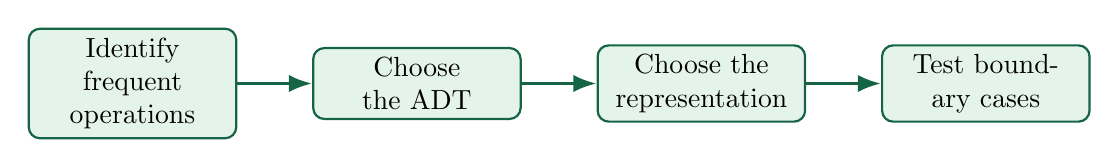
\begin{tikzpicture}[node distance=0.95cm]
  \node[smallbox] (op) {Identify frequent operations};
  \node[smallbox,right=of op] (adt) {Choose the ADT};
  \node[smallbox,right=of adt] (rep) {Choose the representation};
  \node[smallbox,right=of rep] (test) {Test boundary cases};
  \draw[arrow] (op) -- (adt);
  \draw[arrow] (adt) -- (rep);
  \draw[arrow] (rep) -- (test);
\end{tikzpicture}
\end{center}
\vspace{0.2em}
\begin{columns}[T,onlytextwidth]
\begin{column}{0.32\textwidth}
\begin{exampleblock}{Need fast indexed access}
Dynamic array $\rightarrow$ Python \texttt{list}.
\end{exampleblock}
\end{column}
\begin{column}{0.32\textwidth}
\begin{exampleblock}{Need FIFO behavior}
Queue ADT $\rightarrow$ \texttt{deque} or linked queue.
\end{exampleblock}
\end{column}
\begin{column}{0.32\textwidth}
\begin{exampleblock}{Need ordered range queries}
Tree-based structure or sorted representation.
\end{exampleblock}
\end{column}
\end{columns}
\end{frame}

\begin{frame}{Self-check: ADTs and implementations}
\small
\begin{enumerate}
  \item A program needs to undo the most recent editing command. Which ADT is natural?
  \item A system retrieves student records by student ID. Which Python structure is natural?
  \item A report needs all IDs in increasing order and range queries such as IDs between 1000 and 1999. Why might an ordered structure be better than a hash set?
  \item Why is a stack not the same thing as a Python list?
  \item Which advanced structure family is commonly used for database indexes: BST, heap, or B-tree?
\end{enumerate}
\begin{block}{Discussion rule}
For each answer, name the required operation before naming the data structure.
\end{block}
\end{frame}

\begin{frame}{Key takeaways}
\small
\begin{itemize}
  \item Data structures should be chosen from the operations required by the workload.
  \item An ADT describes behavior and operations; an implementation describes memory representation.
  \item Core structures include arrays/lists, linked lists, stacks, queues, deques, dictionaries/maps, and sets.
  \item Advanced structures include tree families, BSTs, balanced BSTs, heaps, B-trees/B+ trees, tries, and graphs.
  \item Python provides built-in and standard-library containers, but linked structures and trees are often implemented explicitly when needed for learning or custom behavior.
  \item The design workflow is: identify operations $\rightarrow$ choose ADT $\rightarrow$ choose implementation.
\end{itemize}
\end{frame}

\end{document}
